% !TEX encoding = UTF-8 Unicode
\documentclass[
11pt,
master, % тип документа
subf, % подключить и настроить пакет subfig для вложенной нумерации рисунков
href, % подключить и настроить пакет hyperref
colorlinks=true, % цветные гиперссылки
times, % шрифт Times как основной
%fixint=false % отключить прямые знаки интегралов
]{disser}
\usepackage[table,xcdraw]{xcolor} % цвет в таблицах
\usepackage[left=25mm, top=20mm, right=10mm, bottom=20mm]{geometry}
\usepackage[T2A]{fontenc}
\usepackage[utf8]{inputenc}
\usepackage[english,russian]{babel}
\usepackage{amsmath,amssymb,cmap} % cmap для кодировки шрифтов в pdf
\usepackage{pdfpages} % вставляем pdf файлы
\usepackage{indentfirst} % отделять первую строку раздела абзацным отступом
\usepackage{titletoc} % убираем отступ перед "Оглавление"
\usepackage{graphicx}
\usepackage{setspace}
\usepackage{verbatim} % для оформления кода
\usepackage{pdfsync} % установка соответствия документ - код
\graphicspath{{./Img/}}
\setlength\parindent{5ex} % абзацный отступ равный пяти строчным буквам основного шрифта
\pagestyle{plain} % включаем нумерацию
\setcounter{tocdepth}{2} % включать подсекции в оглавление
\linespread{1.3} % полуторный интервал
\setcounter{tocdepth}{3} %%where n is the level, starting with 0 (chapters only)

% Номера страниц снизу и по центру
\pagestyle{footcenter}
\chapterpagestyle{footcenter}

\begin{document}

\pagestyle{empty}
\begin{center}

\noindent  Федеральное государственное бюджетное образовательное учреждение\\
высшего профессионального образования\\

Московский государственный технический университет им. Н.Э. Баумана \\
Факультет <<Фундаментальные науки>>\bigskip\\

\vfill

Лабораторная работа №10\\
по курсу «Вычислительная физика»\\
Тема: «Приближённые методы решения краевых задач для ОДУ»\\
\textbf{Вариант 6}\\


\vfill
\vfill
\begin{flushright}
\begin{tabular}{ll}
Выполнили: & студенты группы ФН4-72Б     \\
           & Хижик А.И., Мистрюкова Л.А. \\
Проверил:  & доцент, к.физ.-мат.н.       \\
           & Хасаншин Р.Х.
\end{tabular}
\end{flushright}
\vfill
\begin{center}
Москва, $2019$
\end{center}

\end{center}
\pagebreak


\pagestyle{plain}
\tableofcontents

\section{Теоретическая часть}
\subsection{Метод прогонки}
Для систем алгебраических уравнений метод прогонки -- аналог метода Гаусса. Используется для решения систем с разреженными матрицами, а именно, трёхдиагональными матрицами.

Пусть требуется найти решение следующей системы трёхточечных уравнений:
\begin{equation}\label{eq1}
\left\{
  \begin{array}{ll}
    c_0 y_0 - b_0 y_1 = f_0, & \hbox{$i = 0$,} \\
    -a_i y_{i-1} + c_i y_i - b_i y_{i+1} = f_i, & \hbox{$1 \leq i \leq n - 1$,} \\
    -a_n y_{n-1} + c_n y_n = f_n, & \hbox{$i = n$,}
  \end{array}
\right.
\end{equation}
или в векторном виде
$$\mathcal{A}Y = F,$$
где $Y = (y_0,\ldots,y_n)$ -- вектор неизвестных, $F = (f_0,\ldots,f_n)$ -- вектор правых частей, $\mathcal{A}$ -- квадратная $(n+1) \times (n+1)$ матрица,
$$\mathcal{A} = \left(
  \begin{array}{ccccc}
    c_0 & -b_0 & \ldots & 0 & 0 \\
    -a_1 & c_1 & \ldots & 0 & 0 \\
    0 & 0 & \ldots & 0 & 0 \\
    0 & 0 & \ldots & c_{n-1} & -b_{n-1} \\
    0 & 0 & \ldots & -a_n & c_n \\
  \end{array}
\right).$$

Системы вида (\ref{eq1}) возникают при трёхточечной аппроксимации краевых задач для обыкновенных дифференциальных уравнений второго порядка с постоянными и переменными коэффициентами, а также при реализации разностных схем для уравнений в частных производных. В последнем случае обычно требуется решить не единичную задачу (\ref{eq1}), а серию задач с различными правыми частями, причем число задач в серии может равняться нескольким десяткам и сотням при числе неизвестных в каждой задаче $n \approx 100$. Поэтому необходимо разработать экономичные методы решения задач вида (\ref{eq1}), число действий для которых пропорционально числу неизвестных. Для системы (\ref{eq1}) таким методом является метод прогонки.

Возможность построения экономичного метода заключена в специфике системы (\ref{eq1}). Соответствующая (\ref{eq1}) матрица $\mathcal{A}$ принадлежит к классу разреженных матриц из $(n+1)^2$ элементов ненулевыми являются не более $3n + 1$ элементов. Кроме того, она имеет ленточную структуру (является трёхдиагональной матрицей). Такое регулярное расположение ненулевых элементов матрицы $\mathcal{A}$ позволяет получить очень простые расчётные формулы для вычисления решения.

Введем обозначения, полагая $\alpha_1 = \frac{b_0}{c_0}$, $\beta_1 = \frac{f_0}{c_0}$, и запишем (\ref{eq1}) в следующем виде:
\begin{equation}\label{eq2}
\left\{
  \begin{array}{ll}
    y_0 - \alpha_1 y_1 = \beta_1, & \hbox{$i = 0$,} \\
    -a_i y_{i-1} + c_i y_i - b_i y_{i+1} = f_i, & \hbox{$1 \leq i \leq n - 1$,} \\
    -a_n y_{n-1} + c_n y_n = f_n, & \hbox{$i = n$.}
  \end{array}
\right.
\end{equation}

Из первых двух уравнений (\ref{eq2}) получим
$$y_1 - \alpha_2 y_2 = \beta_2,\;\;\alpha_2 = \frac{b_1}{c_1 - \alpha_1 a_1},\;\;\beta_2 = \frac{f_1 + a_1 \beta_1}{c_1 - \alpha_1 a_1}.$$

В результате имеем <<укороченную>> систему
\begin{equation}\label{eq3}
\left\{
  \begin{array}{ll}
    y_1 - \alpha_2 y_2 = \beta_2, & \hbox{$i = 1$,} \\
    -a_i y_{i-1} + c_i y_i - b_i y_{i+1} = f_i, & \hbox{$2 \leq i \leq n - 1$,} \\
    -a_n y_{n-1} + c_n y_n = f_n, & \hbox{$i = n$,}
  \end{array}
\right.
\end{equation}
которая не содержит неизвестное $y_0$ и имеет аналогичную (\ref{eq2}) структуру. Если эта система будет решена, то неизвестное $y_0$ найдется по формуле $y_0 = \alpha_1 y_1 + \beta_1$. К системе (\ref{eq3}) можно снова применить описанный способ исключения неизвестных. В результате $l$-го шага получим систему для неизвестных $y_l,\ldots, y_n$:
\begin{equation}\label{eq4}
\left\{
  \begin{array}{ll}
    y_l - \alpha_{l+1} y_{l+1} = \beta_{l+1}, & \hbox{$i = l$,} \\
    -a_i y_{i-1} + c_i y_i - b_i y_{i+1} = f_i, & \hbox{$l+1 \leq i \leq n - 1$,} \\
    -a_n y_{n-1} + c_n y_n = f_n, & \hbox{$i = n$,}
  \end{array}
\right.
\end{equation}
и формулы для нахождения $y_i$ с номерами $i \leq l-1$
\begin{equation}\label{eq5}
    y_i = \alpha_{i+1} y_{i+1} + \beta_{i+1},\;\;i = \overline{l-1,\ldots,0},
\end{equation}
Коэффициенты $\alpha_i$ и $\beta_i$ находятся по формулам
$$\alpha_1 = \frac{b_0}{c_0},\;\;\beta_1 = \frac{f_0}{c_0},$$
$$\alpha_{i+1} = \frac{b_i}{c_i - a_i \alpha_i},\;\;\beta_{i+1} = \frac{f_i + a_i \beta_i}{c_i - a_i \alpha_i},\;\;i = \overline{1, n-1},$$
Полагая в (\ref{eq5}) $l = n - 1$, получим систему для $y_n$ и $y_{n-1}$
$$y_{n-1} - \alpha_n y_n = \beta_n,\;\; y_{n-1} + c_n y_n = f_n,$$
из которой найдем $y_n = \beta_{n+1}$, $y_{n-1} = \alpha_n y_n + \beta_n$.

Объединяя эти равенства с (\ref{eq5}) получим окончательные формулы для нахождения неизвестных
 \begin{equation}\label{eq6}
    y_i = \alpha_{i+1} y_{i+1} + \beta_{i+1},\;\;i = \overline{n-1,\ldots,0},
\end{equation}
$$y_n = \beta_{n+1},$$
где $\alpha_i$ и $\beta_i$ находятся по рекуррентным формулам
 \begin{equation}\label{eq7}
    \alpha_{i+1} = \frac{b_i}{c_i - a_i \alpha_i},\;\; i = \overline{1, n-1},\;\;\alpha_1 = \frac{b_0}{c_0},
\end{equation}
\begin{equation}\label{eq8}
    \beta_{i+1} = \frac{f_i + a_i \beta_i}{c_i - a_i \alpha_i},\;\; i = \overline{1, n},\;\; \beta_1 = \frac{f_0}{c_0}.
\end{equation}

Формулы (\ref{eq6}-\ref{eq8}) описывают метод Гаусса, который в применении к системе (\ref{eq1}) получил специальное название -- метод прогонки. Коэффициенты $\alpha_i$, $\beta_i$ называют прогоночными коэффициентами, формулы (\ref{eq7}-\ref{eq8}) описывают прямой ход прогонки, а (\ref{eq6}) -- обратный ход. Так как значения $y_i$ находятся здесь последовательно при переходе от $i + 1$ к $i$, то формулы (\ref{eq6}-\ref{eq8}) называют иногда формулами правой прогонки.

Элементарный подсчёт арифметических действий в (\ref{eq6}-\ref{eq8}) показывает, что реализация метода прогонки по этим формулам требует выполнения $3n$ умножений, $2n + 1$ делений и $3n$ сложений и вычитаний. Если не делать различия между арифметическими операциями, то общее их число для метода прогонки есть $Q = 8n+1$. Из этого числа $3n - 2$ операции затрачиваются на вычисление $\alpha_i$ и $5n + 3$ операций на вычисление $\beta_i$ и $y_i$.

Несложно заметить, что коэффициенты $\alpha_i$ не зависят от правой части системы (\ref{eq1}), а определяются только коэффициентами разностных уравнений $a_i$, $b_i$, $c_i$. Поэтому, если требуется решить серию задач (\ref{eq1}) с различными правыми частями, но с одной и той же матрицей $\mathcal{A}$, то прогоночные коэффициенты $\alpha_i$ вычисляются только при решении первой задачи из серии. Для каждой последующей задачи определяются только коэффициенты $\beta_i$ и решение $y_i$, причём используются найденные ранее $\alpha_i$. Таким образом, на решение только первой из серии задач тратится число арифметических действий $Q = 8n + 1$, на решение каждой следующей задачи будет затрачиваться уже только $5n + 3$ операции.

В заключение укажем порядок счёта по формулам метода прогонки. Начиная с $\alpha_1$ и $\beta_1$, по формулам (\ref{eq7}) и (\ref{eq8}) определяются и запоминаются прогоночные коэффициенты $\alpha_i$ и $\beta_i$. Затем по формулам (\ref{eq6}) находится решение $y_i$.

\textbf{Лемма 1}. Пусть коэффициенты системы (\ref{eq1}) действительны и удовлетворяют условиям $|b_0| \geq 0$, $|a_n| \geq 0$, $|c_0| > 0$, $|c_n| > 0$, $|a_i| > 0$, $|b_i| > 0$, $i = \overline{1, n-1}$,
\begin{equation}\label{eq9}
    |c_i| \geq |a_i| + |b_i|, \;\; i = \overline{1, n-1},
\end{equation}
\begin{equation}\label{eq10}
    |c_0| \geq |b_0|, \;\; |c_n| \geq |a_n|,
\end{equation}
причём хотя бы в одном из неравенств (\ref{eq9}) или (\ref{eq10}) выполняется строгое неравенство, т. е. матрица $\mathcal{A}$ имеет диагональное преобладание. Тогда для алгоритма (\ref{eq6}-\ref{eq8}) метода прогонки имеют место неравенства $c_i - a_i \alpha_i \neq 0$, $\alpha_i \leq 1$, $i = \overline{1,n}$ гарантирующие корректность и устойчивость метода.

\subsection{Применение метода прогонки для решения ОДУ}
Рассмотрим линейное ДУ второго порядка
\begin{equation}\label{eq11}
    L[y] = y'' + p(x) y'(x) + q(x) y(x) = f(x)
\end{equation}
на интервале $x\in[a,b]$ с краевыми условиями
\begin{equation}\label{eq12}
    l_0[y] = \varkappa_1 y(a) + \varkappa_2 y'(a) = f_0,
\end{equation}
$$l_1[y] = \nu_1 y(b) + \nu_2 y'(b) = f_n.$$

Введем на $[a,b$] равномерную сетку $x_i = a + ih$, $i = \overline{0, n}$ и заменим (\ref{eq11}-\ref{eq12}) следующей разностной задачей:
\begin{equation}\label{eq13}
    \frac{y_{i+1} - 2y_i + y_{i-1}}{h^2} + \frac{p_i(y_{i+1} - y_{i-1})}{2h} + q_i y_i = f_i,
\end{equation}
\begin{equation}\label{eq14}
    \varkappa_1 y_0 + \varkappa_2 \frac{y_1 - y_0}{h} = f_0,
\end{equation}
$$\nu_1 y_n + \nu_2 \frac{y_n - y_{n-1}}{h} = f_n.$$

Преобразуем выражения (\ref{eq13}-\ref{eq14}) к виду:
$$\left\{
  \begin{array}{ll}
    C_0 y_0 - B_0 y_1 = f_0, & \hbox{$i = 0$,} \\
    -A_i y_{i-1} + C_i y_i - B_i y_{i+1} = f_i, & \hbox{$1 \leq i \leq n-1$,} \\
    -A_n y_{n-1} + C_n y_n = f_n, & \hbox{$i = n$,}
  \end{array}
\right.$$
где
$$C_0 = \varkappa_1 - \frac{\varkappa_2}{h},\;\; B_0 = - \varkappa_2,$$
$$A_i = \frac{p_i}{2h} - \frac{1}{h^2}, \;\; C_i = \frac{2}{h^2} - q_i, \;\; B_i = -\frac{1}{h^2} - \frac{p_i}{2h},$$
$$A_n = \frac{\nu_2}{h}, \;\; C_n = \nu_1 + \frac{\nu_2}{h}.$$

\subsection{Методы минимизации невязки при решения краевых задач для ОДУ}
Рассмотрим линейное ДУ второго порядка
\begin{equation}\label{eq15}
    L[y] = y'' + p(x)y' + q(x)y = f(x),\;\; x\in[a,b]
\end{equation}
с граничными условиями
\begin{equation}\label{eq16}
    l_a[y] = \alpha_0 y(a) + \beta_0 y'(a) = A,
\end{equation}
$$l_b[y] = \alpha_1 y(b) + \beta_1 y'(b) = B.$$

\textbf{Утверждение.} Краевая задача (\ref{eq15}-\ref{eq16}) имеет единственное решение, если соответствующая однородная задача имеет только тривиальное решение.

\subsubsection{Метод коллокации}
Будем искать приближённое решение линейной краевой задачи (\ref{eq15}-\ref{eq16}) в виде функции
\begin{equation}\label{eq17}
    y_n(x) = \varphi_0(x) + \sum_{i=1}^{n}c_i \varphi_i(x),
\end{equation}
где определяемые на отрезке $[a,b]$ базисные функции $\varphi_i(x)$, $i = \overline{1,n}$ и дополнительная функция $\varphi_0(x)$ должны быть дважды дифференцируемыми и попарно линейно независимыми. Кроме того, функция $\varphi_0(x)$ должна удовлетворять данным краевым условиям (\ref{eq16}), а функции $\varphi_i(x)$ при $i = \overline{1,n}$ -- соответствующим однородным краевым условиям, т.е. должны выполняться равенства
\begin{equation}\label{eq18}
\left\{
  \begin{array}{ll}
    \alpha_0 \varphi_i(a) + \alpha_1 \varphi'_i(a) = 0, & \hbox{$\forall i \in \mathbb{N}$}, \\
    \beta_0 \varphi_i(b) + \beta_1 \varphi'_i(b) = 0.
  \end{array}
\right.
\end{equation}

В таком случае функция $y_n(x)$, определяемая выражением (\ref{eq17}), при любых значениях коэффициентов $c_i$ гарантированно удовлетворяет краевым условиям (\ref{eq16}).

Представление приближённого решения $y_n(x)$, подобное (\ref{eq17}), характерно для многих приближенно-аналитических методов решения краевых задач; главное их различие состоит в том, на какой основе ищутся коэффициенты $c_i$ в линейной комбинации базисных функций $\varphi_i(x)$ выражения (\ref{eq17}).

В методе коллокации коэффициенты $c_i$ в представлении (\ref{eq17}) приближённого решения $y_n(x)$ подбираются так, чтобы в узлах коллокации $x_i$ таких, что
$$a < x_1 < \ldots < x_n < b,$$
значения $y_n(x_i)$ приближённого решения были согласованы с точными значениями $y(x_i)$.

Поскольку точное решение $y(x)$ неизвестно, согласование $y_n(x)$ с $y(x)$ в узлах коллокации $x_i$ проводим подстановкой $y_n(x)$ в уравнение (\ref{eq15}). Получаем равенство
\begin{equation}\label{eq19}
    y''_n(x_i) + p(x_i) y'_n(x_i) + q(x_i)y_n(x_i) = f(x_i),
\end{equation}
которое, в силу выставляемого требования согласования $y_n(x_i)$ с $y(x_i)$, считаем точным при каждом $i = \overline{1,n}$. Продифференцировав дважды функцию $y_n(x)$ в представлении (\ref{eq17}), от равенства (\ref{eq19}) переходим к равенству
\begin{equation}\label{eq20}
    \sum_{j=1}^{n} c_j \varphi''_j(x_i) + p_i \sum_{j=1}^{n} c_j \varphi_j'(x_i) = f_i - \varphi''_0(x_i) - p_i \varphi'_0(x_i) - q_i \varphi_0(x_i).
\end{equation}
Положим
\begin{equation}\label{eq21}
    a_{ij} = \varphi''_j(x_i) + p_i\varphi'_j(x_i) + q_i \varphi_j(x_i),
\end{equation}
\begin{equation}\label{eq22}
    b_i = f_i - \varphi''_0(x_i) - p_i \varphi'_0(x_i) - q_i \varphi_0(x_i).
\end{equation}
Тогда (\ref{eq20}) приобретает стандартный вид линейной алгебраической системы
\begin{equation}\label{eq23}
    \sum_{j=1}^{n} a_{ij}c_j = b_i, \;\; i = \overline{1, n}
\end{equation}
относительно коэффициентов $\{c_i\}$.

Успех применения метода коллокации к задаче (\ref{eq15}-\ref{eq16}), впрочем, как и других приближенно-аналитических методов, сильно зависит от удачного выбора базисных функций $\varphi_i(x)$ в представлении приближённого решения (\ref{eq17}). В конкретных задачах выбор таких функций, по возможности, должен опираться на априорные или эмпирические сведения о решении.

\subsubsection{Интегральный метод наименьших квадратов}
Метод основан на минимизации интеграла
\begin{equation}\label{eq32}
I = \int_{a}^{b} \psi^2(x, c_1, \ldots, c_n) dx,
\end{equation}
где $\psi(x, c_1, \ldots, c_n) = L[y_n(x)] - f(x) = L[\varphi_0(x)] + \sum_{i=1}^{n} c_i L[\varphi_i(x)] - f(x)$ -- невязка точного и приближённого решений. Условие минимума $I$:
$$\int_{a}^{b} \psi \frac{\partial \psi}{\partial c_i} = 0, \;\; i = \overline{1,n},$$
\begin{equation}\label{eq33}
\left\{
  \begin{array}{ll}
    c_1(L[\varphi_1], L[\varphi_1]) + \ldots + c_n(L[\varphi_n], L[\varphi_1]) = (f - L[\varphi_0], L[\varphi_1]),\\
    \ldots\\
    c_1(L[\varphi_1], L[\varphi_n]) + \ldots + c_n(L[\varphi_n], L[\varphi_n]) = (f - L[\varphi_0], L[\varphi_n]).
  \end{array}
\right.
\end{equation}

Система (\ref{eq33}) имеет единственное решение, если $\{L[\varphi_i]\}$ образуют линейно независимую систему функций.

Определитель Грамма, построенный на базе скалярных произведений системы (\ref{eq33}), равен нулю, если функции линейно зависимы.
\subsubsection{Дискретный метод наименьших квадратов}

Метод основан на минимизации суммы
\begin{equation}\label{eq34}
\sum_{i=1}^{n} \psi^2(x_i, c_1, \ldots, c_n), \;\; x_i \in (a,b).
\end{equation}

Если в качестве скалярного произведения использовать $(f,g) = \sum_{i=1}^{n} f(x_i)g(x_i)$, то получим систему (\ref{eq33}).

\subsubsection{Метод подобластей}

Пусть $x_i \in [a,b]$. Потребуем, чтобы

$$\int_{x_{i-1}}^{x_i} \psi(x, c_1, \ldots, c_n)dx = 0, \;\; i = \overline{1,n}.$$

\subsubsection{Метод Галёркина}
Пусть $L$ -- некоторый линейный оператор, действующий в гильбертовом пространстве $\mathcal{H}$, т.е. в полном нормированном пространстве со скалярным произведением $(\circ, \circ)$. Стоит задача приближённого решения операторного уравнения
\begin{equation}\label{eq24}
    L[y] = f,
\end{equation}
т.е. задача отыскания некоторого приближения к неизвестному элементу $y \in \mathcal{H}$, соответствующему заданному элементу $f \in \mathcal{H}$. Пусть, далее, $\{\varphi_i(x)\}_{i=1}^\infty$ -- некоторая полная замкнутая система линейно независимых элементов из $\mathcal{H}$. Ее $n$ первых элементов $\{\varphi_i\}_{i=1}^n$ выделяют в $\mathcal{H}$ конечномерное подпространство $\mathcal{H}_n$, в котором и ищется приближённое решение уравнения (\ref{eq24}):
\begin{equation}\label{eq25}
    y_n = \sum_{i=1}^{n}c_i \varphi_i(x)
\end{equation}

Для удобства будем считать, что элемент $L[y_n]$ принадлежит тому же подпространству $\mathcal{H}_n$. Тогда к тривиальному равенству
$$f = L[y_n] + (f - L[y_n])$$
можно применить одну из центральных теорем теории гильбертовых пространств, согласно которой любой элемент гильбертова пространства может быть представлен в виде суммы определённого элемента подпространства (проекции данного элемента на подпространство) и определённого элемента пространства, ортогонального к выбранному подпространству (реализующего расстояние от исходного элемента до его проекции).

Принадлежность элемента $f - L[y_n]$ ортогональному к $\mathcal{H}_n$ подпространству $\mathcal{H}_n^\perp$ означает, что он ортогонален каждому элементу $\varphi_i$, входящему в базис пространства $\mathcal{H}_n$. Таким образом, при любом $i = \overline{1,n}$ имеем:
$$(f - L[y_n]) \perp \varphi_i \Leftrightarrow (f - L[y_n], \varphi_i) = 0 \Leftrightarrow (L[y_n], \varphi_i) = (f, \varphi_i).$$
Подставляя сюда выражение $y_n$ (\ref{eq25}) и пользуясь простейшими свойствами скалярного произведения, получаем:
\begin{equation}\label{eq26}
    \left(L\left[\sum_{j=1}^{n} c_j \varphi_j\right], \varphi_i\right) = (f, \varphi_i) \Leftrightarrow \sum_{j=1}^{n}(L[\varphi_j], \varphi_i)c_j = (f, \varphi_i).
\end{equation}

Метод Галёркина приближённого решения операторного уравнения (\ref{eq24}) сводится к нахождению коэффициентов $\{c_i\}_{i=1}^n$ линейной комбинации некоторых задаваемых определённым образом линейно независимых функций $\{\varphi_i\}_{i=1}^n$ так, чтобы эти коэффициенты удовлетворяли линейной системе
\begin{equation}\label{eq27}
\sum_{j=1}^{n} a_{ij}c_j = d_i, \;\; i = \overline{1,n},
\end{equation}
где
\begin{equation}\label{eq28}
a_{ij} = (L[\varphi_j], \varphi_i), \;\; d_i = (f, \varphi_i).
\end{equation}

Вернёмся к рассмотрению краевой задачи (\ref{eq15}-\ref{eq16}). Естественным для ее рассмотрения пространством является гильбертово пространство $\mathcal{L}_2[a, b]$ функций, интегрируемых на отрезке $[a,b]$ с квадратом. Скалярное произведение здесь определяется равенством
\begin{equation}\label{eq29}
(u,\upsilon) = \int_{a}^{b} u(x) \upsilon(x) dx.
\end{equation}

Будем искать приближённое решение задачи (\ref{eq15}-\ref{eq16}) в виде задаваемой формулой (\ref{eq17}) функции $y_n(x)$ такой, чтобы она удовлетворяла данным краевым условиям, а это будет, как мы уже знаем, если
$$l_a[\varphi_0] = A, \;\; l_b[\varphi_0] = B,$$
$$l_a[\varphi_i] = 0, \;\; l_b[\varphi_i] = 0, \;\; \forall i = \overline{1,n}.$$
Подставляя $y_n(x)$ в данное уравнение (\ref{eq15}), в силу линейности определённого там дифференциального оператора $L[y]$, имеем:
$$L\left[\varphi_0 + \sum_{i=1}^{n} c_i \varphi_i\right] = f \Leftrightarrow L\left[\sum_{i=1}^{n} c_i \varphi_i\right] = f - L[\varphi_0].$$
Следовательно, в таком случае, наличие дополнительного слагаемого $\varphi_0$ в представлении приближённого решения (\ref{eq17}) вместо представления (\ref{eq25}) означает, что равенство (\ref{eq26}) нужно переписать в виде
$$\left(L\left[\sum_{i=1}^{n} c_j \varphi_j\right], \varphi_i\right) = (f - L[\varphi_0], \varphi_i),$$
а это, в свою очередь, вносит поправку в выражение $d_i$, зафиксированное равенством (\ref{eq28}). Согласно этому замечанию и определению (10.61) скалярного произведения, находим выражение свободного члена $d_i$ $i$-го уравнения системы (\ref{eq28}):
\begin{equation}\label{eq30}
d_i = (f - L[\varphi_0], \varphi_i) = \int_{a}^{b}[f(x) - \varphi''_0(x) - p(x)\varphi'_0(x) - q(x)\varphi_0(x)] \varphi_i(x) dx.
\end{equation}

Выразим коэффициенты СЛАУ (\ref{eq27}) в соответствии с записанной в (\ref{eq28}) формулой:
\begin{align*}
	a_{ij} &= (L[\varphi_i], \varphi_i) = \int_{a}^{b}[\varphi''_j(x) + p(x) \varphi'_j(x) + q(x) \varphi_j(x)] \varphi_i(x) dx = \\
	& =  \int_{a}^{b} \varphi''_j (x) \varphi_i(x) dx + \int_{a}^{b} p(x) \varphi'_j(x) dx + \int_{a}^{b} q(x) \varphi_j(x) \varphi_i(x) dx.
\end{align*}
Преобразуем <<по частям>> первый интеграл в выражении и получим
\begin{equation}\label{eq31}
a_{ij} = \varphi_i(b)\varphi'_j(b) - \varphi_i(a)\varphi'_j(a) - \int_{a}^{b} \varphi'_j(x)\varphi'_i(x) dx + \int_{a}^{b} p(x) \varphi'_j(x)\varphi_i(x) dx + \int_{a}^{b} q(x) \varphi_j(x)\varphi_i(x) dx.
\end{equation}
Выполненное преобразование интеграла, во-первых, активизировало роль краевых условий при построении приближённого решения $y_n(x)$ в форме (\ref{eq17}), во-вторых, позволило ослабить требования к гладкости базисных функций $\varphi_i(x)$, поскольку теперь, как видно из (\ref{eq31}), у них могут быть даже разрывы производных. Подмеченный факт говорит о том, что методом Галёркина при подходящем выборе базисных функций можно находить решения краевых задач, определённые в каком-либо обобщённом смысле.

\newpage
\section{Постановка задачи}
\begin{itemize}
\item Решить краевую задачу $y'' + y' - 2y= 0$, $x\in [0,1]$, $y(0) = 2$, $y(1) = \exp(1) + \exp(2)$, используя метод прогонки.
\item Аппроксимировать функцию Рунге с помощью кубического сплайна при глобальном способе задания наклонов, используя метод прогонки для решения системы для определения наклонов.
\item Решить краевую задачу $L[y] = y'' + \left(1+x^2\right)y = -1$, $x\in [-1,1]$, $y(-1) = 0$, $y(1) = 0$. Базисные функции: $\varphi_0(x) = 0$, $\varphi_i (x) = x^{2i-2}\left(1 - x^2\right)$, $i\in \mathbb{N}$. Точки коллокации: $x_0 = 0$, $x_1 = -\frac{1}{2}$, $x_2 = \frac{1}{2}$. Приближённое решение искать в виде: $y_2(x) = c_1 \left(1 - x^2\right) + c_2 x^2\left(1 - x^2\right)$.

Решить краевую задачу, используя интегральный и дискретный метод наименьших квадратов.
\item Решить краевую задачу $L[y] = y'' + y = -x$, $x \in [0,1]$, $y(0) = 0$, $y(1) = 0$, используя метод Галеркина. Базисные функции: $\varphi_0(x) = 0$, $\varphi_i(x) = x^i (1-x)$, $i\in \mathbb{N}$. Найти приближённые решения $y_2$ и $y_3$.
\end{itemize}


\newpage
\section{Программа}
\subsection{Задание А}
{\footnotesize
\begin{verbatim}
#include <iostream>
#include <math.h>
using namespace std;

class NDSolve{
private:
    double *a, *b, *x, *D;
    double left_b, right_b, cond1, cond2, A, B, C, p, q, h;
    int size;
public:
    NDSolve(double in1, double in2, double l, double r, double p1, double q1){
        size = 10;
        a = new double[size+1];
        b = new double[size+1];
        x = new double[size+1];
        D = new double[size];
        left_b = l;
        right_b = r;
        cond1 = in1;
        cond2 = in2;
        h = (right_b - left_b)/(size-1);
        p = p1;
        q = q1;
    }
    void CreateMatrix();
    void Reverse_stroke();
    void Forward_stroke();
    double Function(double t);
};

int main(){
    NDSolve object(2, exp(1) + exp(-2), 0, 1, 1, -2);
    object.CreateMatrix();
    object.Forward_stroke();
    object.Reverse_stroke();
    return 0;
}

double NDSolve::Function(double t){
    return 0;
}
void NDSolve::CreateMatrix(){
    B =  (0.5*p*h + 1);
    C = (-2 + q*h*h);
    A =  (-0.5*p*h + 1);
    for(int i = 0; i < size;i++){
        D[i] = h*h*Function(left_b + h*i);
    }
}
void NDSolve::Forward_stroke(){
    a[1] = 0;
    b[1] = cond1;
    for (int i = 1; i < size - 1; i++) {
        a[i + 1] = -1 * B / (C + A * a[i]);
        b[i + 1] = (D[i] - A * b[i]) / (C + A * a[i]);
    }
}
void NDSolve::Reverse_stroke(){
    x[size-1] = cond2;
    cout << "{{" << (size-1)*h << ", " << x[size-1] << "}";
    for (int i = size-1; i > 0; i--) {
        x[i - 1] = a[i] * x[i] + b[i];
        cout << ", {" << (i - 1)*h << ", " << x[i-1] << "}";
    }
}
\end{verbatim}
}

\newpage
\subsection{Задание Б}
\footnotesize{
\begin{verbatim}
#include <iostream>
using namespace std;

class Spline{
private:
    double *a, *b, *m, *D;
    double left_b, right_b, A{}, B{}, C{}, h;
    int size;
public:
    explicit Spline(int N){
        size = N;
        a = new double[size+1];
        b = new double[size+1];
        m = new double[size+1];
        D = new double[size];
        left_b = -1;
        right_b = 1;
        h = (right_b - left_b)/(size-1);
    }
    void CreateMatrix();
    void Reverse_stroke();
    void Forward_stroke();
    double Values(double x, int index);
    void Spline1();
    static double R(double t);
};
double Spline::R(double t){
    return  1.0 / (1.0 + 25.0 * t * t);
}
void Spline::CreateMatrix(){
    B =  1.0;
    C = 4.0;
    A =  1.0;
    D[0] = (-11*R(left_b) + 18*R(left_b + h) - 9*R(left_b + 2*h) + 2*R(left_b + 3*h))/h/6.0;
    for(int i = 1; i < size-1;i++){
        D[i] = 3*(R(left_b + h*(i+1))  - R(left_b + h*(i-1)))/h;
    }
    D[size-1] = (11*R(right_b) - 18*R(right_b - h) + 9*R(right_b - 2*h) - 2*R(right_b - 3*h))/h/6.0;
}
void Spline::Forward_stroke(){
    a[1] = 0;
    b[1] = R(-1);
    for (int i = 1; i < size - 1; i++) {
        a[i + 1] = -1 * B / (C + A * a[i]);
        b[i + 1] = (D[i] - A * b[i]) / (C + A * a[i]);
    }
}
void Spline::Reverse_stroke(){
    m[size-1] = R(1);
    for (int i = size-1; i > 0; i--) {
        m[i - 1] = a[i] * m[i] + b[i];
    }
}
double Spline::Values(double x, int index){
    double data_x[size+1];
    double data_y[size + 1];

    for (int i = 0; i <= size; i++){
        data_x[i] = left_b + h*i;
        data_y[i] = R(left_b + h*i);
    }
    double s1, s2, s3, s4;
    double xi = data_x[index];
    double xii = data_x[index + 1];
    s1 = (pow((xii - x), 2) * (2 * (x - xi) + h)) * data_y[index] / (h*h*h);
    s2 = (pow((x - xi), 2) * (2 * (xii - x) + h)) * data_y[index + 1] /  (h*h*h);
    s3 = pow((xii - x), 2) * (x - xi) * m[index] /  (h*h);
    s4 = pow((x - xi), 2) * (x - xii) * m[index + 1] /  (h*h);
    return s1 + s2 + s3 + s4;
}
void Spline::Spline1(){
    int M = 25;
    for(int i = 0; i <= size-2; i++){
        for(int j = 0; j <= M; j++){
            cout << "{" << left_b + i*h + j*h/M << ", " << Values(left_b + h * i + h / M * j, i) << "}, ";
        }
    }
}
int main(){
    Spline object(5);
    object.CreateMatrix();
    object.Forward_stroke();
    object.Reverse_stroke();
    object.Spline1();
    return 0;
}

\end{verbatim}
}

\newpage
\section{Результаты вычислений}
\subsection{Задание А}
\begin{figure}[h]
\begin{minipage}[h]{1\linewidth}
\center{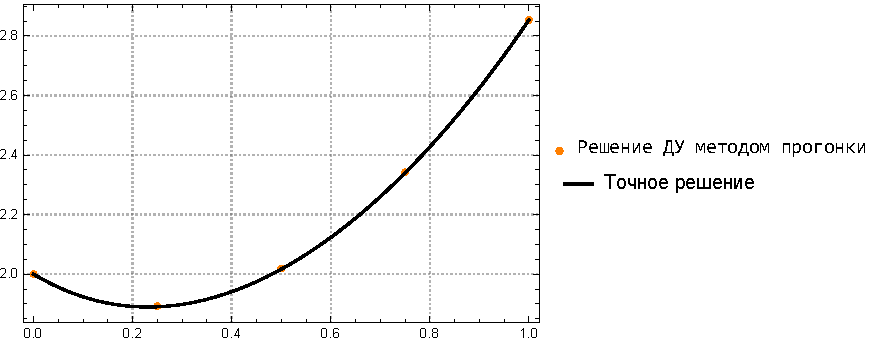
\includegraphics[width=0.8\linewidth]{plS1_5.pdf}} a) \\
\end{minipage}
\vfill
\begin{minipage}[h]{1\linewidth}
\center{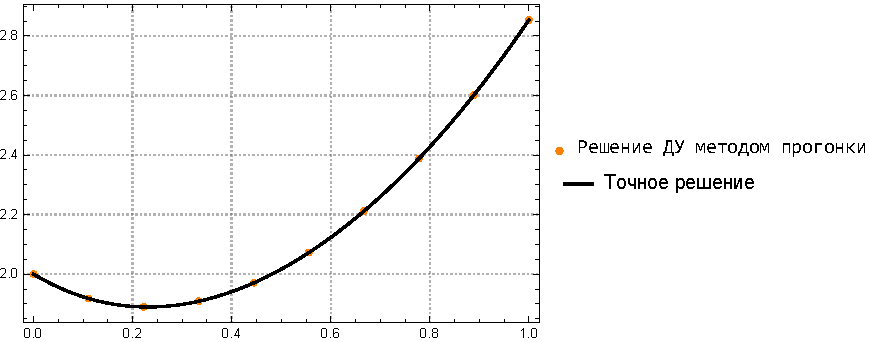
\includegraphics[width=0.8\linewidth]{plS1_10.pdf}} b) \\
\end{minipage}
\vfill
\begin{minipage}[h]{1\linewidth}
\center{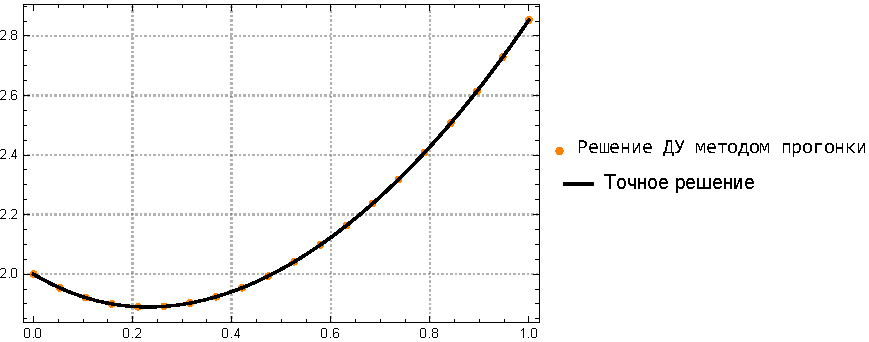
\includegraphics[width=0.8\linewidth]{plS1_20.pdf}} c) \\
\end{minipage}
\caption{Точное и численное решения краевой задачи $y'' + y' - 2y = 0$, $x \in [0,1]$, $y(0) = 2$, $y(1) = \exp(1) + \exp(2)$ методом прогонки для  a) $N = 5$, b) $N = 10$, с) $N = 20$.}
\label{ris:1}
\end{figure}

\newpage
\subsection{Задание Б}
\begin{figure}[h!]
\begin{minipage}[h]{1\linewidth}
\center{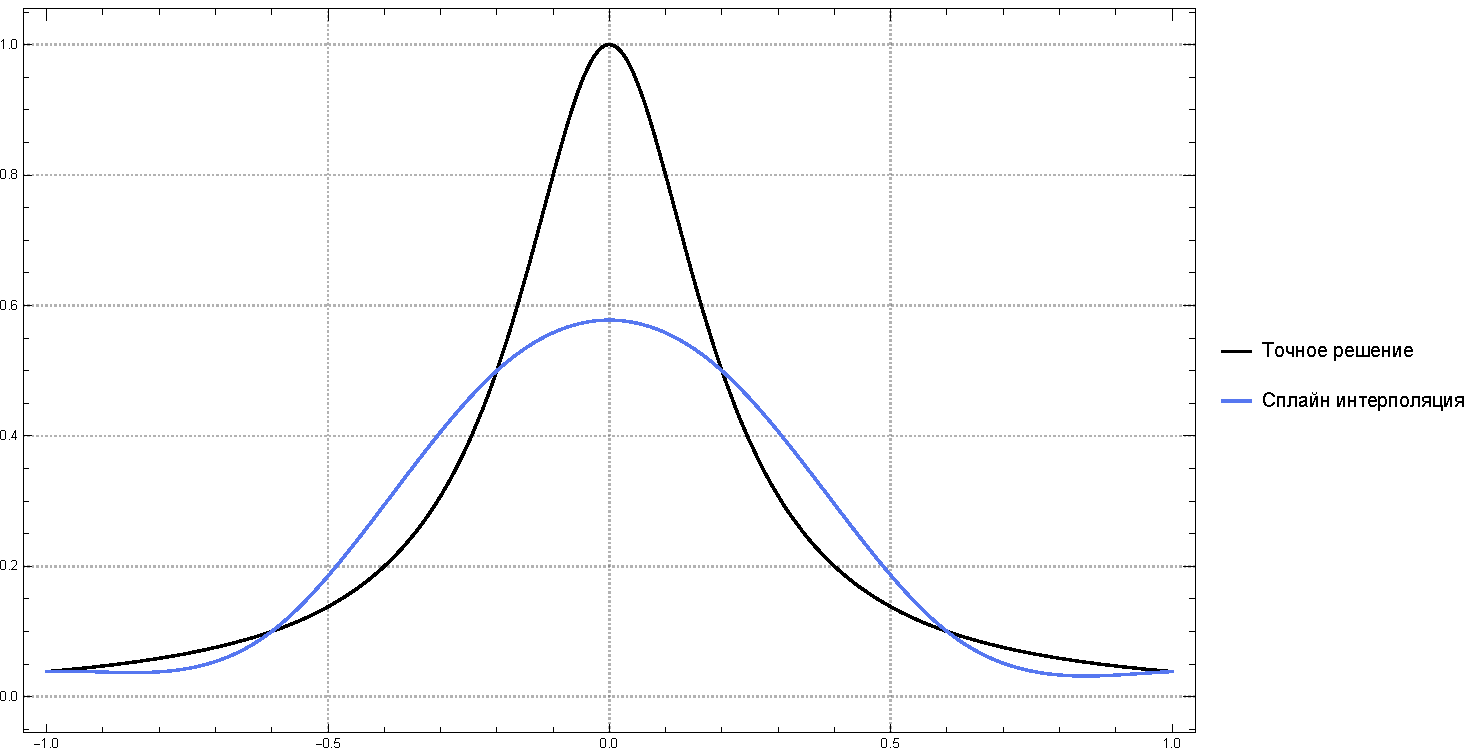
\includegraphics[width=0.8\linewidth]{plS2_5.pdf}} a) \\
\end{minipage}
\vfill
\begin{minipage}[h]{1\linewidth}
\center{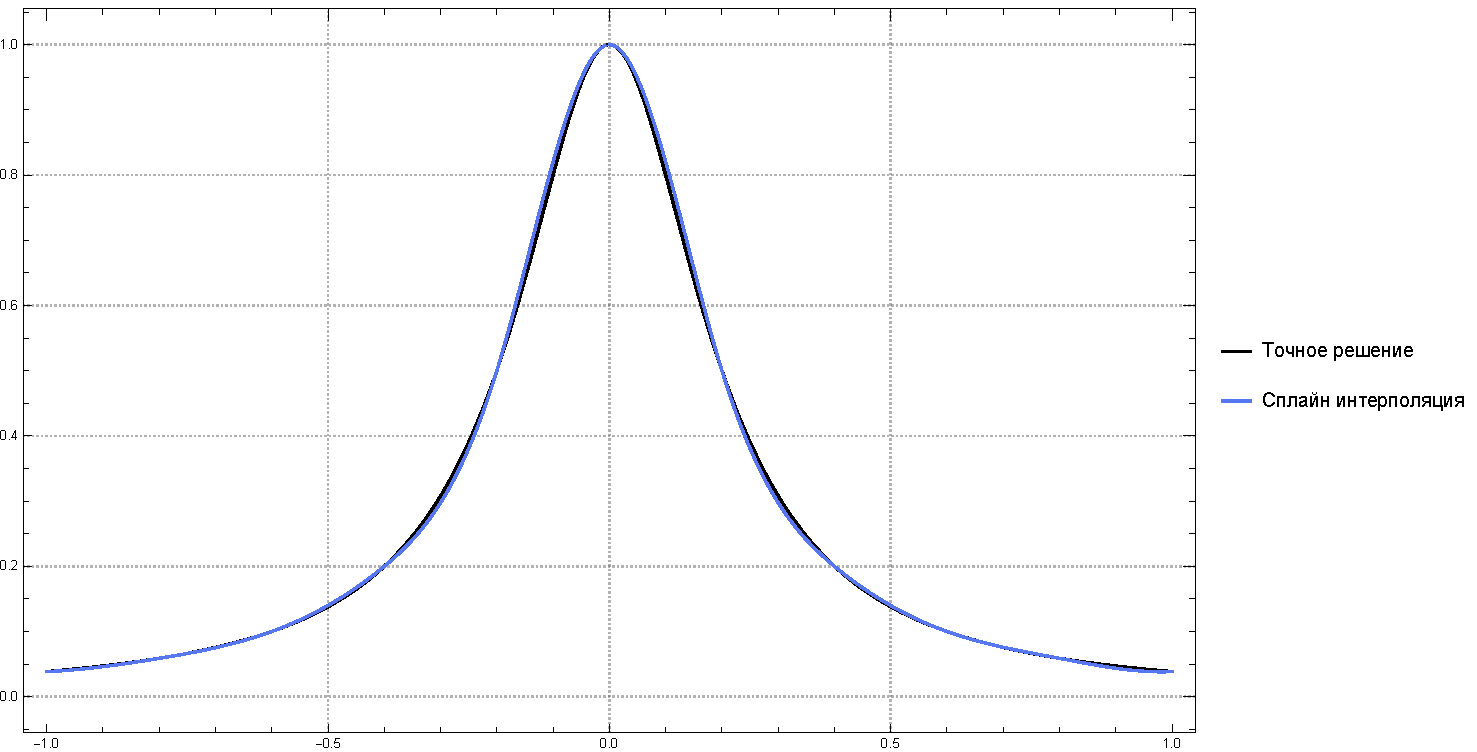
\includegraphics[width=0.8\linewidth]{plS2_10.pdf}} b) \\
\end{minipage}
\vfill
\begin{minipage}[h]{1\linewidth}
\center{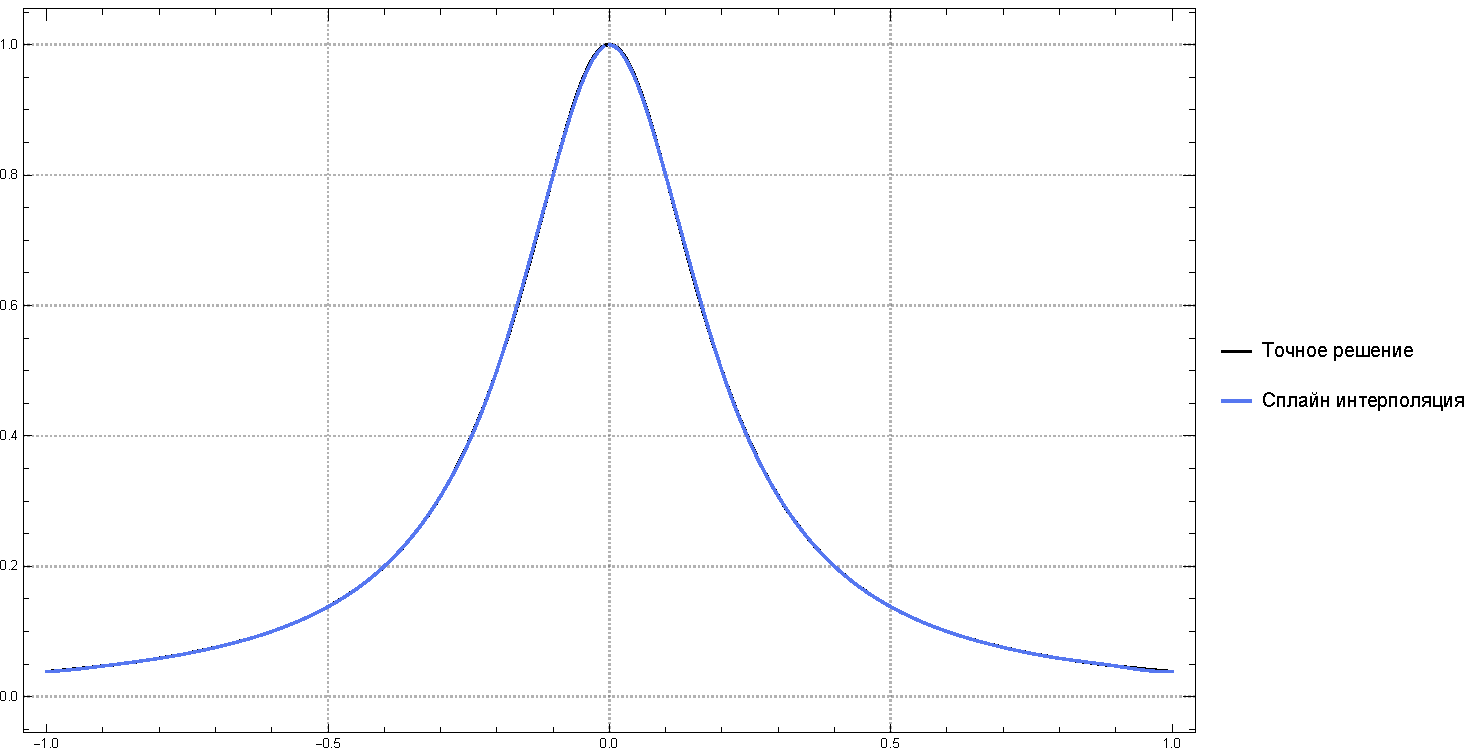
\includegraphics[width=0.8\linewidth]{plS2_20.pdf}} c) \\
\end{minipage}
\caption{Аппроксимация функции Рунге $f(x) = \frac{1}{1 + 25 x^2}$ кубическими сплайнами при глобальном способе задании наклонов для a) $N = 5$, b) $N = 10$, с) $N = 20$ частичных отрезков.}
\label{ris:2}
\end{figure}

\subsection{Задание В}
\textbf{Аппроксимирующие функции}
\begin{itemize}
  \item Метод коллокации:
  $$y(x) = \frac{16}{17} \left(1-x^2\right).$$
  \item Интегральные метод наименьших квадратов:
  $$y(x) = \frac{31755933}{34046644} \left(1-x^2\right) - \frac{2321319}{34046644} x^2 \left(1-x^2\right).$$
  \item Дискретный метод наименьших квадратов:
  $$y(x) = \frac{16}{17} \left(1-x^2\right).$$
\end{itemize}

\begin{figure}[h]
  \centering
  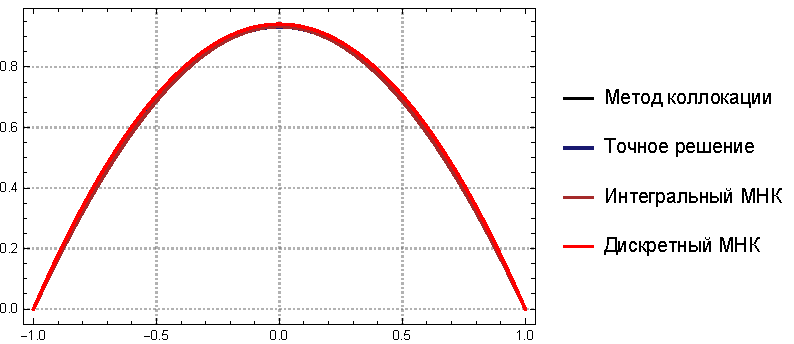
\includegraphics[width=0.8\linewidth]{plS3.pdf}
  \caption{Точное и численное решения краевой задачи $L[y] = y'' + \left(1+x^2\right)y = -1$, $x\in [-1,1]$, $y(-1) = 0$, $y(1) = 0$ для базисных функций $\varphi_0(x) = 0$, $\varphi_i (x) = x^{2i-2}\left(1 - x^2\right)$, $i\in \mathbb{N}$ и точек коллокации $x_0 = 0$, $x_1 = -\frac{1}{2}$, $x_2 = \frac{1}{2}$ при использовании метода коллокации, интегрального и дискретного МНК.}\label{ris:3}
\end{figure}

\newpage
\subsection{Задание Г}
\textbf{Аппроксимирующие функции}
\begin{itemize}
  \item Метод Галеркина для $n = 2$:
  $$y_2(x) = \frac{71}{369} x(1-x) + \frac{7}{41} x^2 (1-x).$$
  \item Метод Галеркина для $n = 3$:
  $$y_3(x) = \frac{13811}{73554} x(1-x) + \frac{2380}{12259} x^2 (1-x) - \frac{7}{299} x^3 (1-x).$$
\end{itemize}

\begin{figure}[h]
  \centering
  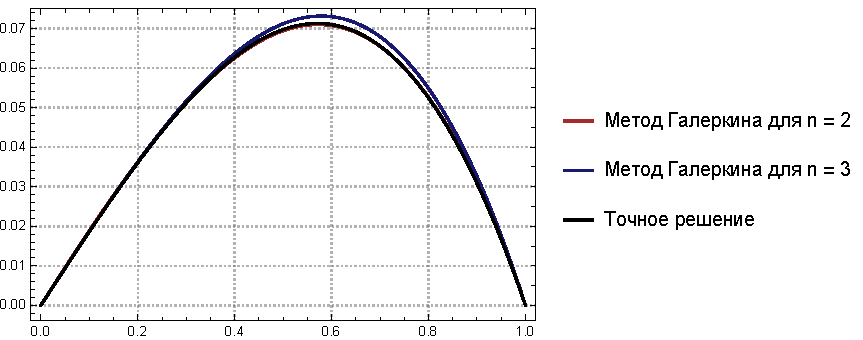
\includegraphics[width=0.8\linewidth]{plS4.pdf}
  \caption{Точное и численное решение краевой задачи $L[y] = y'' + y = -x$, $x \in [0,1]$, $y(0) = 0$, $y(1) = 0$ для базисных функций $\varphi_0(x) = 0$, $\varphi_i(x) = x^i (1-x)$, $i\in \mathbb{N}$ при использовании метода Галеркина}\label{ris:4}
\end{figure}


\newpage
\section{Вывод}
В лабораторной работе рассмотрены такие способы решения краевых задач, как метод прогонки, метод коллокации, интегральный и дискретный методы наименьших квадратов и метод Галеркина; была получена аппроксимация функции Рунге $f(x) = \frac{1}{1 + 25 x^2}$ с помощью кубического сплайна при глобальном способе задания наклонов.

Точность метода Галеркина значительно возросла при использовании большего числа базисных функций. При решении краевой задачи $L[y] = y'' + \left(1+x^2\right)y = -1$, $x\in [-1,1]$, $y(-1) = 0$, $y(1) = 0$ для базисных функций $\varphi_0(x) = 0$, $\varphi_i (x) = x^{2i-2}\left(1 - x^2\right)$, $i\in \mathbb{N}$ и точек коллокации $x_0 = 0$, $x_1 = -\frac{1}{2}$, $x_2 = \frac{1}{2}$ методом коллокации, интегральным и дискретным МНК, наибольшую точность показал интегральный МНК.
\end{document} 